\begin{document}

\maketitle

\section{Sissejuhatus}
\begin{frame}[fragile]
  \frametitle{Eelmine kord}
  Saame tuttavaks ja räägime strateegiast üldiselt
	\begin{itemize}
		\item Sissejuhatus: kes ma olen ja kuidas minu käest hinde saab
		\item IT seos äristrateegiaga, IT mõju ärile
		\item Süsteemidest ja tarkvara arhitektuurist
	\end{itemize}
\end{frame}

\begin{frame}[fragile]
  \frametitle{Täna kavas}
		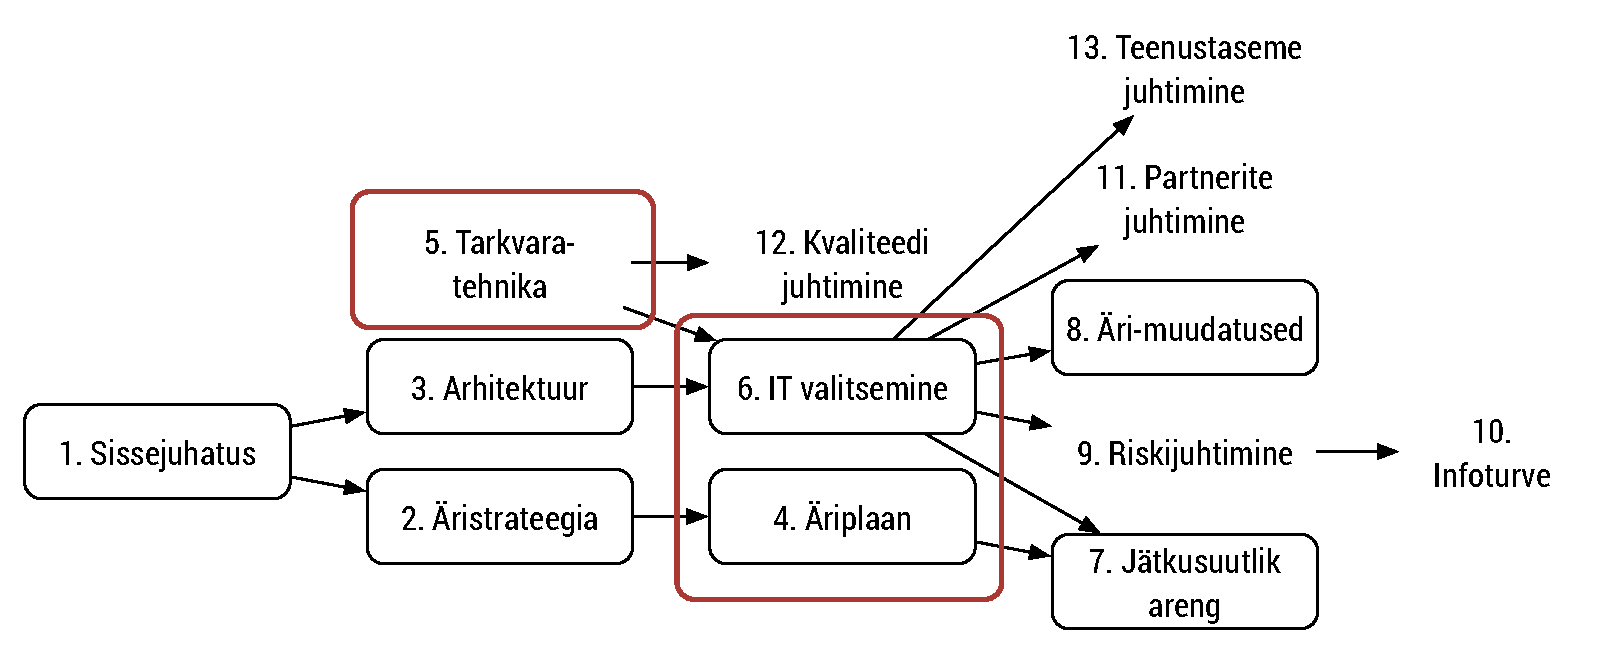
\includegraphics[width=\textwidth]{aine_struktuur_teine.pdf}
\end{frame}

\section{Äriplaani koostamine}
\begin{frame}[fragile]
  \frametitle{IT Kulud}
  	ITle kulutatakse raha vaid siis, kui see aitab aktsionäridele väärtust luua. Järelikult:
	\begin{itemize}
		\item On täiesti normaalne, et ITle kulutatav kõigub
		\item On IT-juhi töö näidata, kuidas iga kulutatud euro aktsionäridele väärtust loob
		\note{Mitte lihtsalt väärtust, vaid väärtust aktsionäridele\\}
		\item IT-juhi töö on disainida ärimudelile vastav IT organisatsioon, mitte vastupidi
	\end{itemize}
\end{frame}

\begin{frame}[fragile]
  \frametitle{Arenduse ja halduse kulud}
  	\begin{columns}[t]
		\begin{column}[T]{6.5cm}
			\begin{itemize}
				\item Halduskulud on funktsioon eelmise perioodi halduskuludest ja \emph{eelmise perioodi arenduskuludest}
				\item Tehniline võlg tuleb tellija juurest ja läheb tellija juurde saades vahepeal IT probleemiks
				\item Kui $A_{vana}=0$, siis H kasvab isegi, kui $A_n=const$
			\end{itemize}
		\end{column}
		\begin{column}[T]{3.5cm}
			\begin{align}
				K_n &= H_n+A_n \nonumber \\
			    H_n &= H(H_{n-1}, A_{n-1}, I_n) \nonumber\\
			    A_n &= A_{uus}(A_{n-1}, I_n) \nonumber \\
			    &\quad {} + A_{vana}(A_{n-1}, I_n) \nonumber
		    \end{align}
		\end{column}
	\end{columns}
\end{frame}
\note{Kuna IT väärtust tajutakse sageli just läbi uute arenduste järeldub siit, et kui vana ja uue arenduse suhe on vale, väheneb konstantsete investeeringute puhul IT võimekus uut tajutud väärtust tooota.}

\begin{frame}[fragile]
  \frametitle{Järeldused}
	\begin{itemize}
		\item On strateegiliselt oluline kliendile seletada tänaste otsuste mõju homsetele kuludele
		\item Tarkvara kapitaliseerimise otsused on IT-juhile elutähtsad
		\item IT-juhi jaoks on oluline olla kapitaliseerimisotsuste juures laua taga
	\end{itemize}
\end{frame}
\note{Et olla kapitaliseerimisotsuste juures laua taga, peab IT-juht suutma seal tõsiseltvõetavalt kaasa rääkida}


\begin{frame}[fragile]
  \frametitle{Arhitektuur ja äri}
  	\begin{center}
			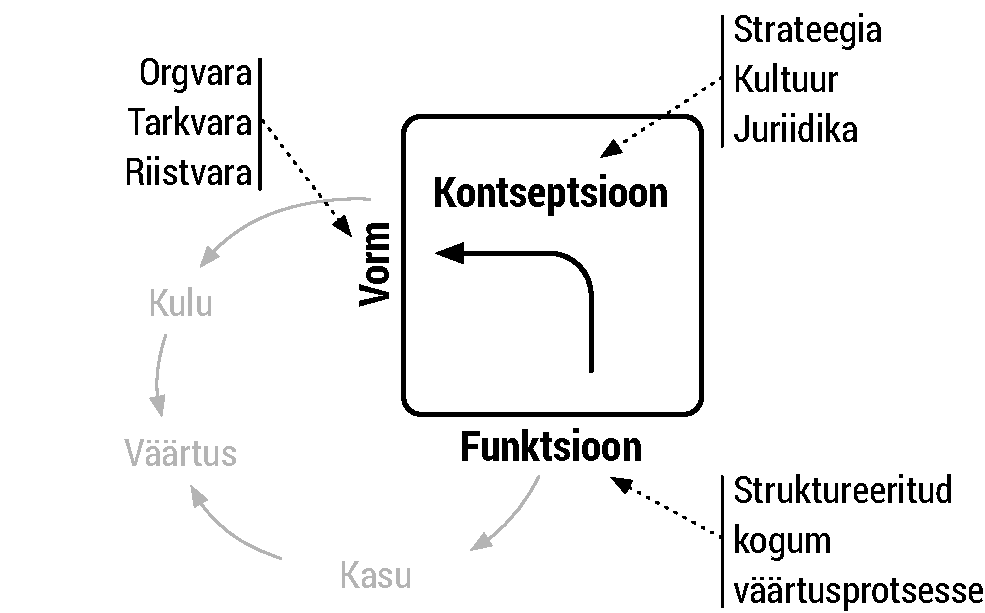
\includegraphics[width=.7\textwidth]{ffc_profit.pdf}
	\end{center}
\end{frame}

\begin{frame}[fragile]
	\frametitle{Arhitektuur ja äri}
			\begin{itemize}
				\item Arhitektuur määrab toote või teenuse \emph{võimekuse} kasumit teenida
				\item Sealhulgas
				\begin{itemize}
					\item Tootmiskulud. Kui kallist programmerijat teie arhitektuur eeldab?
					\item Halduskulud. Kas olemasolevad adminid tulevad toime?
					\item Väljumiskulud. Kui keeruline on teie tarkvarast loobuda?
				\end{itemize}
				\item Arhitekt peab ettevõtte ärimudelist väga hästi aru saama ja suutma tolle arusaamaga midagi ette võtta
			\end{itemize}
\end{frame}
\note{Oluline rõhk võimekusel. Mäletate: arhitektuur määrab vektorid, mille sisustab disain. Kui aga parameetrid on paigast ära, ei tule kasumist midagi. Ehk. Vale arhitektuur tähendab, et äri ei saa olla kasumlik, õige arhitektuur ei tähenda, et äri on kasumlik.}

%Arutelu koht
\begin{frame}[fragile]
  \frametitle{Arutelu koht}
		\begin{center}
			\textbf{Kuidas seletada kliendile, et ta saab sama raha eest täna vähem, kui eile?}
		\end{center}
\end{frame}

\section{Tarkvaratehnika}
\begin{frame}[fragile]
  \frametitle{Tarkvaratehnika definitisioon}
	\begin{center}
		\begin{quote}
			Tarkvaratehnika on süstemaatiline lähenemine tarkvara analüüsile, disainile, hindamisele, realiseerimisele, testimisele, haldamisele ja ümbertöötamisele, ehk, inseneriteaduse rakendamine tarkvarale.
		\end{quote}		
	\end{center}
	\cite{laplante}
\end{frame}
\note{Väga asjalik raamat, nii palju kui sirvida jõudsin. Annab kena ülevaate, mis üldse tarkvaratehnikas toimub}

\begin{frame}[fragile]
  \frametitle{Definitsiooni järelmid}
	\begin{itemize}
		\item Mainitud seitset eri distsipliini, realisatsioon on vaid üks neist
		\note{Siit peaks tulema vihje rõhuasetuste kohta: enamasti keskendutakse programmeerimisele\\}
		\item Ei ole viidet arendusprotsessile, kui sellisele
			\begin{itemize}
				\item Distsipliine saab kokku panna väga mitmel eri viisil, milline on parim?
				\item Igapäevases elus saab arendusprotsess disproportsionaalselt palju tähelepanu
				\note{Sest kvarteti liikmeid ümber paigutada on lihtne, mõistliku testimisraamistiku välja töötamine aga väga keeruline\\}
			\end{itemize}
		\item Kenasti on kaetud tarkvara elutsükkel, ümbertöötamine (ingl. \emph{reengineering}) on samuti osa protsessist ja oluline kuluallikas
	\end{itemize}
\end{frame}
\note{Programmeerijad on tarkvaratehnika kaaperdanud tõmmates tähelepanu endale ja jättes varju teised valdkonnad. Mis, muidugi, võtavad ära suurema osa ka nende päevast kuid siiski kutsutakse neid 'programmeerijateks'}

\begin{frame}[fragile]
  \frametitle{Tarkvaratehnika olulisus}
  Äristrateegia on otseselt seotud valitud viisiga tarkvara ehitada. Joel \citep{spolsky2004joel2} kirjeldab kenasti Amazon vs. Ben \& Jerry's dilemmat
  \begin{itemize}
  	\item Orgaaniline kasv vs. Ruttu Suureks lähenemine
	\item Head näited tarkvaratehniliste valikute osas
		  \begin{itemize}
		  	\item Kas probleemile lähenetakse raha või mõtlemisega?
			\item Kui oluline on toodetud koodi kvaliteet?
			\item Kas protsess toetab on kiiret rabelemist või jätkusuutlikku arengut?
		  \end{itemize}
	\item Õige vastus sõltub valitud strateegiast. Seega
  \end{itemize}
  \begin{center}
	  \textbf{Otsusta üheselt, kas oled Amazon või Ben \& Jerry's}
  \end{center}
\end{frame}
\note{Lugege Joeli, ta on hea. Suurem osa sisu veebis tasuta saadaval aga raamat on mugavam \par Muidugi on toodud vastuolu vaid üks võimalikke, kuid illustreerib seoseid kenasti}

\begin{frame}[fragile]
  \frametitle{Tarkvaratehnika keerukus}
	Brooks ütleb oma essees \citep{brooks1975mythical}, et \emph{Tarkvara ehitamine on oma olemuselt keeruline}, see ei saa kunagi lihtne olema. 
  \begin{itemize}
	\item Läbi aja on üritatud hõbekuuli siiski leida
		  \begin{itemize}
		  	\item Nõuete kirjeldamine
			\item Mingi protsessi kasutamine
			\item Artefaktide tootmine
			\item "Tagasi loodusse" protsesse eitavad lähenemised
		  \end{itemize}
	\item Keskendu olulisele ja ära lase endale mao-õli müüa
	\note{Tuletage meelde tarkvaratehnika definitsiooni, katsuge igaühte neist võimalikult hästi teha ning siduge tükid kokku nii, nagu mõnus tundub\par
	Ülejäänud Brooks on ka hea, "The mythical man-month" essee peaks olema kohustuslik igale programmeerijaid juhtivale inimesele}
  \end{itemize}
\end{frame}


%Arutelu koht
\begin{frame}[fragile]
  \frametitle{Arutelu koht}
		\begin{center}
			\textbf{Mis teeb programmeerimise keeruliseks?}
		\end{center}
\end{frame}


\begin{frame}[fragile]
  \frametitle{Mõistliku koodi reeglid}
  Mõistliku koodi 12 reeglit \cite{spolsky2004joel}
\small  
	\begin{enumerate}
		\item Kas sa kasutad (mõistlikku) koodikontrolli?
		\item Kas ehitamine on tehtav ühe sammuga?
		\item Kas sa ehitad iga päev?
		\item Kas sul on probleemihoidla?
		\item Kas sa parandad enne uue koodi kirjutamist vead?
		\item Kas sul on kuskil olemas kehtiv projektiplaan?
		\item Kas sul on spetsifikatsioon?
		\item Kas programmeerijatel on rahu ja vaikust?
		\item Kas sa kasutad parimaid tööriistu, mida raha eest saab?
		\item Kas sul on testijad?
		\item Kas uued tulijad kirjutavad intervjuu ajal koodi?
		\item Kas sa teed kiireid kasutatavusteste?
	\end{enumerate}
\normalsize
\end{frame}


\begin{frame}[fragile]
  \frametitle{Tehniline võlg}
	Tehniline võlg tekib, kui mõistliku lahenduse asemel tehakse mittemõistlik. NB! Tegu on \emph{metafooriga} ja tal on piirid.
  \begin{itemize}
	\item Teda võib teatud piirini võrrelda rahalise kohustusega
	\item Ta tuleb investeerida viisil, mis katab hilisemad intressikulud
	\item Tehnilise võla põhjus peaks olema äriline, kuid võib olla ka tehniline 
	\item Vaid ITl on võimekus hallata tehnilise võla portfelli
	\item Tehnilise võla likvideerimisel on reeglina ärilised põhjused kuid võivad olla ka tehnilised
  \end{itemize}

\end{frame}

\begin{frame}[fragile]
  \frametitle{Tehnilise võla kvadrant}
  	\begin{center}
			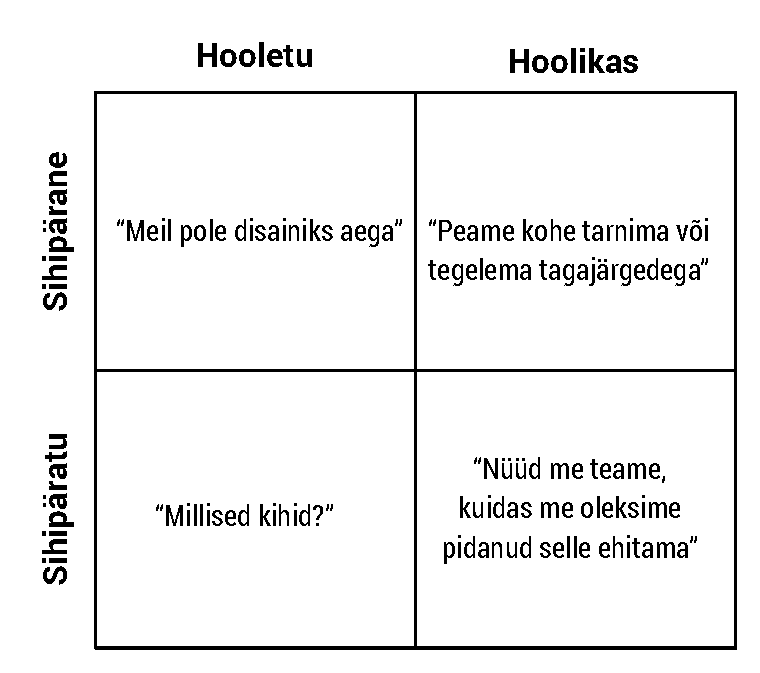
\includegraphics[width=.65\textwidth]{fowler.pdf}
	\end{center}
	\cite{fowlerdebt}
\end{frame}

%Arutelu koht
\begin{frame}[fragile]
  \frametitle{Arutelu koht}
		\begin{center}
			\textbf{Kuidas seletada tehnilist võlga juhtkonnale?}
		\end{center}
\end{frame}

\section{IT valitsemine}

\begin{frame}[fragile]
  \frametitle{IT valitsemine}
  IT valitsemine on olemuselt IT juhtimise administratiivne aspekt
	\begin{itemize}
		\item ITGI definitsioon: ... eestvedamine, organisatsioonilised struktuurid ning protsessid, mis tagavad, et organisatsiooni IT toetab ja laiendab tema strateegiaid ja eesmärke \citep{insitute2003board}
		\item Ühest definitsiooni ei ole, ülejäänud räägivad samuti peamiselt protsessidest, struktuuridest jms. 
		\note{Oluline tõlkeküsimus: leadership, management, governance. Eestvedamine, juhtimine ja valitsemine. Tuleb olla täpne!}
		\item Olulisel kohal on asjade kontrolli all hoidmine ning nende mõjutamine soovitud suunas. 
	\end{itemize}
\end{frame}

\begin{frame}[fragile]
  \frametitle{Poliitikavastasus}
 Ingl. \emph{policy resistance}. Süsteemide omadus suunavatele impulssidele kas mitte reageerida, reageerida vastupidses suunas või naasta mõju lõppedes esialgse olukorra juurde
	\begin{itemize}
		\item Tegemist on põhimõttelise probleemiga, tuleb eristada inimeste käitumist süsteemi käitumisest
		\item Iga süsteem on mingi mõttes tasakaalus, tasakaal võib olla kas stabiilne, ebastabiilne või neutraalne
		\item Kehtib konkreetse poliitika kohta!
		\item Enne poliitika rakendamist või muutmist küsi alati: 
		\begin{itemize}
			\item millised mehhanismid üritavad esialgset olukorda taastada? 
			\item mis tüüpi tasakaalus on mu süsteem?
	\end{itemize}

	\end{itemize}
\end{frame}
\note{Huntide ja jäneste näide. Huntide arvu tõstmiseks tuleb suurendada jäneste juurdekasvu kiirust, mitte lisada hunte}

\begin{frame}[fragile]
  \frametitle{Mida me siis valtseme?}
	Mida me juhime, kui me juhime ITd?
	\begin{itemize}
		\item Inimesi
		\item Ressursse
		\item Protsesse
	\end{itemize}
\end{frame}


%Arutelu koht
\begin{frame}[fragile]
  \frametitle{Arutelu koht}
		\begin{center}
			\textbf{Milline on põhimõtteline vahe IT juhtimise ja IT valitsemise vahel?}
		\end{center}
\end{frame}

\begin{frame}[fragile]
  \frametitle{Inimesed}
  Inimesed käituvad viisil, mis \emph{maksimeerib nende huvisid}. Kuidas need ettevõtte huvidega sobivad, on juhi probleem.
	\begin{itemize}
		\item Jällegi põhimõtteline, mitte konkreetse inimese probleem
		\item Inimeste selline käitumine on oluline poliitikavastasuse allikas 
		\item Enne, kui inimesi valitsema/kontrollima hakata, küsi: 
		\note{Küsida tuleb nimeliselt!\par}
			\begin{itemize}
				\item Kes läheb ära. Need inimesed sa kaotad ja \emph{selliseid enam palgata ning hoida ei õnnestu}
				\item Kes saab edukaks. Neile uus poliitika sobib ja \emph{selliseid hakkab juurde tulema} kas värbamise või olemasolevate muutumise kaudu
				\note{Ülejäänud on kahtlemata olulised, kuid mitte muutuse kontekstis}
			\end{itemize}
	\end{itemize}
\end{frame}

\begin{frame}[fragile]
  \frametitle{Ressursid}
	Ressursid (inimesed, raha, kontor, võrk, jne.) antakse IT juhile \emph{ärilise eesmärgi saavutamiseks}. Ja ainult. Siit kaks kriitilist küsimust:
	\begin{itemize}
		\item Mis see eesmärk on?
		\note{Mõlemast küsimusest peavad aru saama mõlemad\\}
		\item Kui kaugele on antud ressursiga reaalne jõuda?
		\note{Sest ressursse on definitsiooni järgi alati vähe\\}
	\end{itemize}

	Järelikult:
	\begin{itemize}
		\item IT juhi ülesanne on maksimeerida \emph{bang per buck}. 
		\note{Kõik muu on irrelevantne. Seepärast ongi oluline aru saada, mida "bang" antud kontekstis tähendab\\}
		\item peab tehnilise võla juhtimine olema läbipaistev, tellija peab aru saama oma otsuste pikaajalisest mõjust
		\note{Sest tehnilise võla intresside maksmine võtab ressursse, mis on antud sulle ärilise eesmärgi täitmiseks ja mitte võlgade klaarimiseks. Vt. märkus IT juhi valikute kohta}
	\end{itemize}
\end{frame}


\begin{frame}[fragile]
  \frametitle{Protsessid}
	\begin{itemize}
		\item Protsesside valitsemine on klassikaline küberneetilika tagasisidega kontrolli probleem. Anname protsessile sisendi, mõõdame tulemust, võrdleme seda soovituga ja anname uuesti sisendi. 
		\note{Kreeka k. kybernetike "valitsemine"\\}
		\item Tüüpiliselt mõõdetakse tulemi kvaliteeti ja tehtud kulu
		\item Võtmeküsimus: \emph{Kuidas protsesside juhtimist üles skaleerida?}
		\item Spear \citep{spear2010high} väidab, et seda tehes on võimalik eristuda ning saavutada strateegiline eelis
		\note{Spear on hea, vt. ka märkus organisatioonide kiirendamise kohta\\}
		\item Jaapanlastel on hetkel kõige mõistlikum mudel selle küsimuse lahendamiseks. Vt. \emph{Kaizen, muda/mura/muri}
		\note{Agiilsed metoodikad järgivad paljus sama mõtteviisi ning on samuti autotööstuse juurtega (3C projekt)}
	\end{itemize}
\end{frame}


%Arutelu koht
\begin{frame}[fragile]
  \frametitle{Arutelu koht}
		\begin{center}
			\textbf{Kuidas ja miks mõõta programmeerija tulemust?}
		\end{center}
\end{frame}

\begin{frame}[fragile]
  \frametitle{Arenduse sisendi juhtimine}
  \begin{center}
	  Probleem: kuidas otsustada, mis järjekorras tellija soove täita
\bigskip
	\emph{  Ressursse on alati, definitsiooni järgi, vähem, kui vajadusi}
  \end{center}
\end{frame}
	  \note{Kuigi olemuselt taktikaline, on tegu tihti probleemse valdkonnaga. Sellest ka väike kõrvalepõige.}
    
\begin{frame}[fragile]
  \frametitle{Projekti nimekiri kasvab}
  Kui vanni voolab vett kiiremini, kui äravool välja juhib, siis vee tase vannis kasvab.
		\begin{itemize}
			\item Mida pikem on järjekord, seda paindumatum on organisatsioon. 
			\note{Kui meil on nimekirjas kolme aasta jagu projekte, siis nimekirjas viimane jõuab tegemisse kõige varem kolme aasta pärast. Isegi siis, kui arendusvõimekus vastab tellija tellimisvõimekusele\par}
			\item Peab eksisteerima mõistlik mehhanism asjade nimekirjast välja võtmiseks
			\note{Näide nimekirja pikkuse kontrolli kohta: järjekord on fikseeritud pikkusega. kui midagi järjekorda võetakse langeb miski välja\par}
			\item Paberimahuga blokeerimine on vale mõte. Kui tuleb esitada palju dokumentatsiooni, seda hambad ristis, ka tehakse. 
			\note{Tellija vajadus on ju (vähemalt tajutuna) reaalne. Hammaste kriginal tehakse paberid ära. Aga iga nimekirjast välja visatud projekt tähendab raisatud ressursse}				
			\item Projektidel on komme järjekorras hapuks minna
		\end{itemize}
\end{frame}

\begin{frame}[fragile]
  \frametitle{Vältimatu poliitiline surve}
  Eksisteerib vältimatu surve millist iganes rahajagamismehhanismi ümber teha või sellest mööda minna.
		\begin{itemize}
			\item Otsustamine peab olema väga läbipaistev, grupiviisiline ja konsensuslik
			\item Hea mõte on otsustamine mehhaniseerida. 
			\note{Näide otsustamise mehhaniseerimisest: iga üksus saab x koguse raha ja kui see kulutatud, rohkem projekte jutule ei võeta\\}
			\item Mida allpool tehakse otsused, seda vähem poliitiliselt mõjutatavad nad on
			\note{Otsused on mõistlik suruda madalaimale tasemele, kus nii tellija kui täitja poolt on saadaval kogenud mandaadiga juhid, kes omavahel kokku võiksid leppida\\}
			\item Mida sagedasemad on otsused, seda lihtsam on neid teha 
			\note{50 projekti 5 tunniga vs. 5 tunnist koosolekut, igaühes otsustamisel 10 projekti. Kõige parem jooksvad otsused\\}
			\item Peab eksisteerima mõistlik ja kontrollitud viis erandeid teha ilma protsessi diskrediteerimata. 
			\note{Näide erandi tegemise mehhanismist: vanaisa õigus}
		\end{itemize}
\end{frame}

\begin{frame}[fragile]
  \frametitle{Olulised asjad võivad tegemata jääda}
		\begin{itemize}
			\item Pisikesed, kuid olulised muutused (näiteks veaparandused) peab olema võimalik kiiresti ja paindlikult ära teha
			\item See on kriitiline koht tehnilise võla juhtimise seisukohast: tehnilist võlga on peaaegu võimatu tavapärase prioretiseerimise läbi likvideerida 
			\note{Kriitiline võlg on IT, mitte äri valuga. Äri tunneb seda ainult läbi arendusvõimekuse kahanemise ja ei pruugi olla suuteline põhjusi mõistma. Vt. jälle märkust IT juhi valikute kohta\par Mida suuremate "kividega" opereeritakse, seda suuremad tühimikud nende vahele jäävad ja seda ebaefektiivsem on ressursikasutus}
			\item Vt. punkt erandi kohta eelmisel slaidil
		\end{itemize}
\end{frame}


%Arutelu koht
\begin{frame}[fragile]
  \frametitle{Arutelu koht}
		\begin{center}
			\textbf{Mida teha, kui klient ei kuula?}
		\end{center}
\end{frame}


\section{Viited}

\begin{frame}[t,allowframebreaks,]
  	\bibliographystyle{plainnat}
	\bibliography{it_strateegia} 

\end{frame}

%\plain{Küsimusi?}
\begin{frame}[plain]
	\begin{center}Küsimusi?\end{center}
\end{frame}

\end{document}